%%%%(c)
%%%%(c)  This file is a portion of the source for the textbook
%%%%(c)
%%%%(c)    Abstract Algebra: Theory and Applications
%%%%(c)    Copyright 1997 by Thomas W. Judson
%%%%(c)
%%%%(c)  See the file COPYING.txt for copying conditions
%%%%(c)
%%%%(c)
\chap{The Structure of  Groups}{struct}
 

The ultimate goal of group theory is to classify all groups up to
isomorphism; that is, given a particular group, we should be able to
match it up with a known group via an isomorphism. For example, we
have already proved that any finite cyclic group of order $n$ is
isomorphic to ${\mathbb Z}_n$; hence, we ``know'' all finite cyclic
groups. It is probably not reasonable to expect that we will ever know
all groups; however, we can often classify certain types of groups or
distinguish between groups in special cases.  

In this chapter we will characterize all finite abelian groups. We
shall also investigate groups with sequences of subgroups.  If a group
has a sequence of subgroups, say 
\[
G = H_n \supset H_{n-1} \supset \cdots \supset H_1 \supset H_0 = \{ e
\}, 
\]
where each subgroup $H_i$ is normal in $H_{i+1}$ and each of the
factor groups $H_{i+1}/H_i$ is abelian, then $G$ is a solvable group.
In addition to allowing us to distinguish between certain classes of
groups, solvable groups turn out to be central to the study of
solutions to polynomial equations.
 

\section{Finite Abelian Groups}

In our investigation of cyclic groups we found that every group of
prime order was isomorphic to ${\mathbb Z}_p$, where $p$ was a prime
number.  We also determined that ${\mathbb Z}_{mn} \cong {\mathbb Z}_m
\times {\mathbb Z}_n$ when $\gcd(m, n) =1$. In fact, much more is true.
Every finite abelian group is isomorphic to a direct product of cyclic
groups of prime power order; that is, every finite abelian group is
isomorphic to a group of the type 
\[
{\mathbb Z}_{p_1^{\alpha_1}} \times \cdots \times {\mathbb
Z}_{p_n^{\alpha_n}}.
\]

First, let us examine a slight generalization  of finite abelian
groups. Suppose that $G$ is a group and let $\{ g_i\}$ be a set of 
elements in $G$, where $i$ is in some index set $I$ (not necessarily 
finite).  The smallest subgroup of $G$ containing all of the $g_i$'s 
is the subgroup of $G$ \boldemph{generated} by the $g_i$'s. If this 
subgroup of $G$ is in fact all of $G$, then $G$ is generated by the 
set $\{g_i : i \in I \}$. In this case the $g_i$'s are said to be 
the \boldemph{generators}\index{Generators for a 
group}\index{Group!generators of} of $G$. If there is a finite set 
$\{ g_i : i \in I \}$ that generates $G$, then $G$ is \boldemph{finitely 
generated}\index{Group!finitely generated}\index{Finitely generated 
group}.
 
 
\begin{example}{finite_groups}
Obviously, all finite groups are finitely generated. For example, the
group $S_3$ is generated by the permutations $(12)$ and $(123)$. The
group ${\mathbb Z} \times {\mathbb Z}_n$ is an infinite group but is
finitely generated by $\{ (1,0), (0,1) \}$.
\end{example}
 
 
 
\begin{example}{infinite_groups}
Not all groups are finitely generated.  Consider the rational numbers
${\mathbb Q}$ under the operation of addition. Suppose that ${\mathbb Q}$ is
finitely generated with generators $p_1/q_1, \ldots, p_n/q_n$, where
each $p_i/q_i$ is a fraction expressed in its lowest terms.  Let $p$
be some prime that does not divide any of the denominators $q_1,
\ldots, q_n$. We claim that $1/p$ cannot be in the subgroup of ${\mathbb
Q}$ that is generated by  $p_1/q_1, \ldots, p_n/q_n$, since $p$ does
not divide the denominator of any element in this subgroup. This fact
is easy to see since the sum of any two generators is
\[
p_i / q_i + p_j / q_j = (p_i q_j + p_j q_i)/(q_i q_j).
\]
\end{example}
 
 
\begin{theorem}
Let $H$ be the subgroup of a group $G$ that is generated by $\{ g_i
\in G : i \in I \}$. Then $h \in H$ exactly when it is a product of
the form 
\[
h = g_{i_1}^{\alpha_1} \cdots g_{i_n}^{\alpha_n},
\]
where the $g_{i_k}$s are not necessarily distinct.
\end{theorem}
 
 
The reason that powers of a fixed $g_i$ may occur several times in the
product is that we may have a nonabelian group. However, if the group
is abelian, then the $g_i$s need occur only once. For example, a
product such as $a^{-3} b^5 a^7$ could always be simplified (in this
case, to $a^4 b^5$). 
 
 
\medskip
 
 
\begin{proof}
Let $K$ be the set of all products of the form $g_{i_1}^{\alpha_1}
\cdots g_{i_n}^{\alpha_n}$, where the $g_{i_k}$s are not necessarily
distinct. Certainly $K$ is a subset of $H$.  We need only show that
$K$ is a subgroup of $G$. If this is the case, then $K=H$, since $H$ is
the smallest subgroup containing all the $g_i$s.
 
 
Clearly, the set $K$ is closed under the group operation. Since $g_i^0
=1$, the identity is in $K$. It remains to show that the inverse of an
element  $g =g_{i_1}^{k_1} \cdots g_{i_n}^{k_n}$ in $K$ must also be in
$K$. However, 
\[
g^{-1}
= (g_{i_1}^{k_{1}} \cdots g_{i_n}^{k_n})^{-1}
= (g_{i_n}^{-k_n} \cdots g_{i_{1}}^{-k_{1}}).
\]
\end{proof}
%Typo corrected. Suggested by S. Engle. TWJ 11/13/2011
%Subscript numbering corrected.  TWJ 11/17/2012
%Subscript numbering corrected---second try.  TWJ 4/24/2013

\medskip
 
Now let us restrict our attention to finite abelian groups. We can
express any finite abelian group as a finite direct product of cyclic
groups. More specifically, letting $p$ be prime, we define a group $G$
to be a \boldemph{$p$-group}\index{Group!$p$-group} if every element in 
$G$ has as its order a power of $p$. For example, both ${\mathbb Z}_2 
\times {\mathbb Z}_2$ and ${\mathbb Z}_4$ are $2$-groups, whereas 
${\mathbb Z}_{27}$ is a $3$-group. We shall prove that every finite 
abelian group is isomorphic to a direct product of cyclic $p$-groups. 
Before we  state the main theorem concerning finite abelian groups, we 
shall consider a special case.
 
 
\begin{theorem}
Every finite abelian group $G$ is the internal direct product of $p$-groups. 
\end{theorem}


%Changed the statement and proof of the theorem to
%reflect that we are dealing with internal direct products.  TWJ 4/24/2013
 
\begin{proof}
If $|G|= 1$, then the theorem is trivial.  Suppose that the order of
$G$ is greater than 1, say 
\[
|G| = p_1^{\alpha_1} \cdots p_n^{\alpha_n},
\]
where $p_1, \ldots, p_n$ are all prime, and define $G_i$ to be the set
of elements in $G$ of order $p_i^k$ for some integer $k$. Since $G$ is
an abelian group, we are guaranteed that $G_i$ is a subgroup of $G$
for $i = 1, \ldots, n$. We must show that
\[
G = G_1 G_2 \cdots  G_n.
\]
That is, we must be able to write every $g \in G$ as a unique product
$g_{p_1} \cdots g_{p_n}$ where $g_{p_i}$ is of the order of some power
of $p_i$. Since the order of $g$ divides the order of $G$, we know
that 
\[
|g| = p_1^{\beta_1}  p_2^{\beta_2} \cdots p_n^{\beta_n}
\]
for integers $\beta_1, \ldots, \beta_n$. Letting $a_i = |g| /
p_i^{\beta_i}$, the $a_i$'s are relatively prime; hence, there exist
integers $b_1, \ldots, b_n$ such that $a_1 b_1 + \cdots + a_n b_n =
1$. Consequently, 
\[
g = g^{a_1 b_1 + \cdots + a_n b_n} = g^{a_1 b_1} \cdots  g^{a_n b_n}. 
\]
Since
\[
g^{(a_i b_i ) p_i^{\beta_i}} = g^{b_i |g|} = e,
\]
it follows that $g^{a_i b_i}$ must be in $G_{i}$. Let $g_i =
g^{a_i b_i}$. Then $g = g_1 \cdots g_n$ and $G_i \cap G_j = \{ e \}$ for $i
\neq j$. 
 
 
To show uniqueness, suppose that $g = g_1 \cdots g_n = h_1 \cdots h_n$,
with $h_i \in G_i$. Then
\[
e = (g_1 \cdots g_n)(h_1 \cdots h_n)^{-1} = g_1 h_1^{-1} \cdots g_n
h_n^{-1}. 
\]
The order of $g_i h_i^{-1}$ is a power of $p_i$; hence, the order of
$g_1 h_1^{-1} \cdots g_n h_n^{-1}$ is the least common multiple of the
orders of the $g_i h_i^{-1}$.  This must be 1, since the order of the
identity is 1. Therefore, $|g_i h_i^{-1}| =1$ or $g_i =h_i$ for $i =
1, \ldots, n$.
\mbox{\hspace{1in}}
\end{proof}
 
 
\medskip

We shall now state the Fundamental Theorem of Finite Abelian Groups. 
 
 
\begin{theorem}\label{struct:Finite_Abelian_Grps_Theorem}
\textbf{(Fundamental Theorem of Finite Abelian
Groups)}\index{Fundamental Theorem!of Finite Abelian Groups} 
Every finite abelian group $G$ is isomorphic to a direct product of
cyclic groups of the form 
\[
{\mathbb Z}_{p_1^{ \alpha_1 }}
\times
{\mathbb Z}_{p_2^{ \alpha_2 }}
\times
\cdots
\times
{\mathbb Z}_{p_n^{ \alpha_n }}
\]
where the $p_i$'s are primes (not necessarily distinct).
\end{theorem}
 
 
\begin{example}{abelian540}
Suppose that we wish to classify all abelian groups of order $540=2^2
\cdot 3^3 \cdot 5$.  The Fundamental Theorem of Finite Abelian Groups 
tells us that we have the following six possibilities.
\begin{itemize}
 
\item
${\mathbb Z}_2 \times {\mathbb Z}_2 \times {\mathbb Z}_3
\times {\mathbb Z}_3 \times {\mathbb Z}_3 \times {\mathbb Z}_5$;
 
\item
${\mathbb Z}_2 \times {\mathbb Z}_2 \times {\mathbb Z}_3
\times {\mathbb Z}_9 \times {\mathbb Z}_5$;
 
 
\item
${\mathbb Z}_2 \times {\mathbb Z}_2
\times {\mathbb Z}_{27} \times {\mathbb Z}_5$;
 
 
\item
${\mathbb Z}_4 \times {\mathbb Z}_3
\times {\mathbb Z}_3 \times {\mathbb Z}_3 \times {\mathbb Z}_5$;
 
\item
${\mathbb Z}_4 \times {\mathbb Z}_3
\times {\mathbb Z}_9 \times {\mathbb Z}_5$;
 
\item
${\mathbb Z}_4 \times {\mathbb Z}_{27} \times {\mathbb Z}_5$.
 
\end{itemize}
\end{example}
 
The  proof of the Fundamental Theorem relies on the following lemma.

\begin{lemma}\label{struct:lemma:finite_abelian}
Let $G$ be a finite abelian $p$-group and suppose that $g \in G$ has
maximal order. Then $G$ is isomorphic to $\langle g \rangle \times H$
for some subgroup $H$~of~$G$. 
\end{lemma}

%Changed the statement and proof of the theorem to
%reflect that we are dealing with direct products.  Suggested by P. Diethelm.
%TWJ 4/24/2013
 
 
\begin{proof}
Suppose that the order of $G$ is $p^n$.  We shall induct on $n$. If
$n= 1$, then $G$ is cyclic of order $p$ and must be generated by $g$.
Suppose now that the statement of the lemma holds for all integers $k$
with $1 \leq k < n$ and let $g$ be of maximal order in $G$, say
$|g| = p^{m}$.  Then $a^{p^m} = e$ for all $a \in G$. Now choose $h$
in $G$ such that $h \notin \langle g \rangle$, where $h$ has the
smallest possible order.  Certainly such an $h$ exists; otherwise, $G
= \langle g \rangle$ and we are done.  Let $H = \langle h \rangle$.
 
 
We claim that $\langle g \rangle \cap H = \{ e \}$. It suffices to
show that $|H|=p$.  Since $|h^p| = |h| / p$, the order of $h^p$ is
smaller than the order of $h$ and must be in $\langle g \rangle$ by
the minimality of $h$; that is, $h^p = g^r$ for some number $r$.
Hence, 
\[
(g^r)^{p^{m-1}} = (h^p)^{p^{m-1}} = h^{p^{m}} = e,
\]
and the order of $g^r$ must be less than or equal to $p^{m-1}$.
Therefore, $g^r$ cannot generate $\langle g \rangle$.  Notice that $p$
must occur as a factor of $r$, say $r = ps$, and $h^p = g^r = g^{ps}$.
Define $a$ to be $g^{-s}h$. Then $a$ cannot be in $\langle g \rangle$;
otherwise, $h$ would also have to be in $\langle g \rangle$. Also, 
\[
a^p = g^{-sp} h^p = g^{-r} h^p = h^{-p} h^p = e.
\]
We have now formed an element $a$ with order $p$ such that $a \notin
\langle g \rangle$. Since $h$ was chosen to have the smallest order of
all of the elements that are not in $\langle g \rangle$, $|H|  = p$.
 
 
Now we will show that the order of $gH$ in the factor group $G/H$ 
must be the same as the order of $g$ in $G$.  If $|gH| < |g| = 
p^m$, then
\[
H = (gH)^{p^{m-1}} =  g^{p^{m-1}} H;
\]
hence, $g^{p^{m-1}}$ must be in $\langle g \rangle \cap H = \{ e \}$,
which contradicts the fact that the order of $g$ is $p^m$.  Therefore,
$gH$ must have maximal order in $G/H$.  By the Correspondence Theorem
and our induction hypothesis,
\[
G/H \cong \langle gH \rangle \times K/H
\]
for some subgroup $K$ of $G$ containing $H$.  We
claim that $\langle g \rangle \cap K = \{ e \}$. If $b \in \langle g
\rangle \cap K$, then $bH \in \langle gH \rangle \cap K/H =  \{ H \}$ and
$b \in \langle g \rangle \cap H = \{ e \}$. It follows that $G =
\langle g \rangle K$ implies that $G \cong \langle g \rangle \times K$. 
\end{proof}
 
\medskip


The proof of the Fundamental Theorem of Finite Abelian Groups follows
very quickly from Lemma~\ref{struct:lemma:finite_abelian}.  Suppose that $G$ is a finite abelian
group and let $g$ be an element of maximal order in $G$. If $\langle g
\rangle = G$, then we are done; otherwise, $G \cong {\mathbb Z}_{|g|}
\times H$ for some subgroup $H$ contained in $G$ by the lemma.  Since
$|H| < |G|$, we can apply mathematical induction.  
 
 
We now state the more general theorem for all finitely generated
abelian groups.  The proof of this theorem can be found in any of the 
references at the end of this chapter.
 
 
\begin{theorem}
\textbf{(The Fundamental Theorem of Finitely Generated Abelian Groups)}
Every finitely generated abelian group $G$ is isomorphic to a direct
product of cyclic groups of the form 
\[
{\mathbb Z}_{p_1^{ \alpha_1 }}
\times
{\mathbb Z}_{p_2^{ \alpha_2 }}
\times
\cdots
\times
{\mathbb Z}_{p_n^{ \alpha_n }}
\times
{\mathbb Z}
\times \cdots \times
{\mathbb Z},
\]
where the $p_i$'s are primes (not necessarily distinct).
\end{theorem}

 
\section{Solvable Groups}

A \boldemph{subnormal series}\index{Subnormal series of a group} 
of a group $G$ is a finite sequence of subgroups 
\[
G = H_n \supset H_{n-1} \supset \cdots \supset H_1 \supset
H_0 = \{ e \},
\]
where $H_i$ is a normal subgroup of $H_{i+1}$. If each subgroup $H_i$
is normal in $G$, then the series is called a \boldemph{normal
series}\index{Normal series of a group}. The \boldemph{length} of a 
subnormal or normal series is the number of proper inclusions. 
 

\begin{example}{normal_series}
Any series of subgroups of an abelian group is a normal series.
Consider the following  series of groups: 
\begin{gather*}
{\mathbb Z} \supset 9{\mathbb Z} \supset 45{\mathbb Z} \supset 180{\mathbb Z} 
\supset \{0\}, \\
{\mathbb Z}_{24} \supset \langle 2 \rangle \supset \langle 6 \rangle 
\supset \langle 12 \rangle
\supset \{0\}.
\end{gather*}
\end{example}
 
 
\begin{example}{subnormal_series}
A subnormal series need not be a normal series.  Consider the
following subnormal series of the group $D_4$: 
\[
D_4 \supset \{ (1),
(12)(34), (13)(24), (14)(23) \} \supset  \{  (1), (12)(34) \} 
\supset \{ (1) \}.
\]
The subgroup $\{  (1), (12)(34) \}$ is not normal in $D_4$;
consequently, this series is not a normal series.
\end{example}

 
A subnormal (normal) series $\{ K_j \}$ is a \boldemph{refinement of a
subnormal (normal) series} $\{ H_i \}$ if $\{ H_i \} \subset \{ K_j
\}$. That is, each $H_i$ is one of the $K_j$. 
 

\begin{example}{refinement}
The series
\[
{\mathbb Z} \supset 3{\mathbb Z} \supset 9{\mathbb Z} \supset 45{\mathbb Z}
\supset 90{\mathbb Z} \supset 180{\mathbb Z} \supset \{0\}
\]
is a refinement of the series
\[
{\mathbb Z} \supset 9{\mathbb Z} \supset 45{\mathbb Z} \supset 180{\mathbb Z} 
\supset \{0\}.
\]
\end{example}

 
The correct way to study a subnormal or normal series of subgroups,
$\{ H_i \}$ of $G$, is actually to study the factor groups
$H_{i+1}/H_i$.  We say that two subnormal (normal) series $\{H_i \}$
and $\{ K_j \}$ of a group $G$ are \boldemph{isomorphic} if there is a
one-to-one correspondence between the collections of factor groups
$\{H_{i+1}/H_i \}$ and $\{ K_{j+1}/ K_j \}$. 
 

\begin{example}{isomorph_series}
The two normal series
\begin{gather*}
{\mathbb Z}_{60} \supset \langle 3 \rangle \supset  \langle 15 \rangle
\supset \{ 0 \} \\
{\mathbb Z}_{60} \supset \langle 4 \rangle \supset  \langle 20 \rangle
\supset \{ 0 \}
\end{gather*}
of the group ${\mathbb Z}_{60}$ are isomorphic since
\begin{gather*}
{\mathbb Z}_{60} / \langle 3 \rangle \cong \langle 20 \rangle /
\{ 0 \} \cong {\mathbb Z}_{3}
\\
\langle 3 \rangle / \langle 15 \rangle
\cong \langle 4 \rangle /  \langle 20 \rangle \cong {\mathbb Z}_{5}
\\
\langle 15 \rangle / \{ 0 \} \cong {\mathbb Z}_{60} / \langle 4 \rangle
\cong {\mathbb Z}_4.
\end{gather*}
\end{example}
 

A subnormal series $\{ H_i \}$ of a group $G$ is a \boldemph{composition
series}\index{Composition series} if all the factor groups are 
simple; that is, if none of the factor groups of the series contains a
normal subgroup. A normal series $\{ H_i \}$ of $G$ is a \boldemph{
principal series}\index{Principal series} if all the factor groups 
are simple.  
 
 
 
\begin{example}{composition_series}
The group ${\mathbb Z}_{60}$ has  a composition series 
\[
{\mathbb Z}_{60} \supset \langle 3 \rangle \supset  \langle 15 \rangle
\supset \langle 30 \rangle  \supset \{ 0 \}
\]
with factor groups
\begin{align*}
{\mathbb Z}_{60} / \langle 3 \rangle & \cong  {\mathbb Z}_{3} \\
\langle 3 \rangle / \langle 15 \rangle & \cong  {\mathbb Z}_{5} \\
\langle 15 \rangle / \langle 30 \rangle & \cong  {\mathbb Z}_{2} \\
\langle 30 \rangle / \{ 0 \} & \cong  {\mathbb Z}_2.
\end{align*}
Since ${\mathbb Z}_{60}$ is an abelian group, this series is
automatically a principal series. Notice that a composition series
need not be unique.  The series 
\[
{\mathbb Z}_{60} \supset \langle 2 \rangle \supset \langle 4 \rangle 
\supset  \langle 20 \rangle \supset \{ 0 \}
\]
is also a composition series.
\end{example}
 
 
 
\begin{example}{Sn_series}
For $n \geq 5$, the series
\[
S_n \supset A_n \supset \{ (1) \}
\]
is a composition series for $S_n$ since $S_n / A_n \cong {\mathbb Z}_2$
and $A_n$ is simple.
\end{example}
%typo corrected.  Suggested by L. Franklin.
%TWJ - 12/19/2011
 
 
 
\begin{example}{Z_series}
Not every group has a composition series or a principal series.
Suppose that 
\[
\{ 0 \} = H_0 \subset H_1 \subset \cdots \subset H_{n-1}
\subset H_n = {\mathbb Z}
\]
is a subnormal series for the integers under addition. Then $H_1$ must
be of the form $k {\mathbb Z}$ for some $k \in {\mathbb N}$. In this case
$H_1 / H_0 \cong k {\mathbb Z}$ is an infinite cyclic group with many
nontrivial proper normal subgroups. 
\end{example}

%changed n to k in the example.  Suggested by P. Diethelm.
%TWJ 4/24/2013
 
 
 
Although composition series need not be unique as in the case of
${\mathbb Z}_{60}$, it turns out that any two composition series are
related. The factor groups of the two composition series for ${\mathbb 
Z}_{60}$ are ${\mathbb Z}_2$,  ${\mathbb Z}_2$,  ${\mathbb Z}_3$, and  ${\mathbb
Z}_5$; that is,  the two composition series are isomorphic. The
Jordan-H\"{o}lder Theorem says that this is always the case.
 
 
\begin{theorem}[Jordan-H\"{o}lder]\index{Jordan-H\"{o}lder Theorem}
Any two composition series of $G$ are isomorphic.
\end{theorem}
 
 
\begin{proof}
We shall employ mathematical induction on the length of the
composition series.  If the length of a composition series is 1, 
then $G$ must be a simple group.  In this case any two composition
series are isomorphic.
 
 
Suppose now that the theorem is true for all groups having a
composition series of length $k$, where $1 \leq k <n$. Let 
\begin{gather*}
G = H_n \supset H_{n-1} \supset \cdots \supset H_1 \supset
H_0 = \{ e \} \\
G = K_m \supset K_{m-1} \supset \cdots \supset K_1 \supset
K_0 = \{ e \}
\end{gather*}
be two composition series for $G$.  We can form two new subnormal
series for $G$ since $H_i \cap K_{m-1}$ is normal in $H_{i+1} \cap
K_{m-1}$ and $K_j \cap H_{n-1}$ is normal in $K_{j+1} \cap H_{n-1}$:
\begin{gather*}
G = H_n \supset H_{n-1} \supset H_{n-1} \cap K_{m-1} \supset 
\cdots \supset H_0 \cap K_{m-1} = \{ e \} \\
G = K_m \supset K_{m-1} \supset K_{m-1} \cap H_{n-1} \supset 
\cdots \supset K_0 \cap H_{n-1} = \{ e \}.
\end{gather*}
Since $H_i \cap K_{m-1}$ is normal in $H_{i+1} \cap K_{m-1}$, the
Second Isomorphism Theorem (Theorem~\ref{homomorph:theorem:2nd_isomorph}) implies that 
\begin{align*}
(H_{i+1} \cap K_{m-1}) / (H_i \cap K_{m-1}) 
& =  (H_{i+1} \cap K_{m-1}) / (H_i \cap ( H_{i+1} \cap K_{m-1} )) \\
& \cong  H_i (H_{i+1} \cap K_{m-1})/ H_i,
\end{align*}
where $H_i$ is normal in $H_i (H_{i+1} \cap K_{m-1})$. Since $\{ H_i
\}$  is a composition series, $H_{i+1} / H_i$ must be simple;
consequently, $H_i (H_{i+1} \cap K_{m-1})/ H_i$ is either $H_{i+1}/
H_i$ or $H_i/H_i$.  That is, $H_i (H_{i+1} \cap K_{m-1})$ must be
either $H_i$ or $H_{i+1}$. Removing any nonproper inclusions from the
series 
\[
H_{n-1} \supset H_{n-1} \cap K_{m-1} \supset 
\cdots \supset H_0 \cap K_{m-1} = \{ e \}, 
\]
we have a composition series for $H_{n-1}$. Our induction hypothesis
says that this series must be equivalent to the composition series
\[
H_{n-1} \supset \cdots \supset H_1 \supset H_0 = \{ e \}.
\]
Hence, the composition series
\[
G = H_n \supset H_{n-1} \supset \cdots \supset H_1 \supset
H_0 = \{ e \} 
\]
and 
\[
G = H_n \supset H_{n-1} \supset H_{n-1} \cap K_{m-1} \supset 
\cdots \supset H_0 \cap K_{m-1} = \{ e \} 
\]
are equivalent. If $H_{n-1} = K_{m-1}$, then the composition series
$\{H_i \}$ and $\{ K_j \}$ are equivalent and we are done; otherwise,
$H_{n-1} K_{m-1}$  is a normal subgroup of $G$ properly containing
$H_{n-1}$.  In this case $H_{n-1} K_{m-1} = G$ and we can apply the
Second Isomorphism Theorem once again; that is,
\[
K_{m-1} / (K_{m-1} \cap H_{n-1}) \cong (H_{n-1} K_{m-1}) / H_{n-1} =
G/H_{n-1}.
\]
Therefore,
\[
G = H_n \supset H_{n-1} \supset H_{n-1} \cap K_{m-1} \supset 
\cdots \supset H_0 \cap K_{m-1} = \{ e \}
\]
and 
\[
G = K_m \supset K_{m-1} \supset K_{m-1} \cap H_{n-1} \supset 
\cdots \supset K_0 \cap H_{n-1} = \{ e \}
\]
are equivalent and the proof of the theorem is complete.
\end{proof}
 
 
\medskip
 
 
A group $G$ is \boldemph{solvable}\index{Group!solvable} if it has 
a composition series $\{ H_i \}$ such that all of the factor groups 
$H_{i+1} / H_i$ are abelian. Solvable groups will play a fundamental 
role when we study Galois theory and the solution of polynomial 
equations. 
 
 
 
\begin{example}{solvable}
The group $S_4$ is solvable since
\[
S_4 \supset A_4 \supset \{ (1), (12)(34), (13)(24), (14)(23) \} 
\supset \{ (1) \}
\]
has abelian factor groups; however, for $n \geq 5$ the series
\[
S_n \supset A_n \supset \{ (1) \}
\]
is a composition series for $S_n$ with a nonabelian factor group.
Therefore, $S_n$ is not a solvable group for $n \geq 5$. 
\end{example}
 
 
 
 
\markright{EXERCISES}
\section*{Exercises}
\exrule
 
 
 
{\small
\begin{enumerate}
 
\item
Find all of the abelian groups of order less than or equal to 40 up to
isomorphism.
 
\item
Find all of the abelian groups of order 200 up to isomorphism.
 
\item
Find all of the abelian groups of order 720 up to isomorphism.
 
\item
Find all of the composition series for each of the following groups.
\begin{multicols}{2}
\begin{enumerate}

\item
${\mathbb Z}_{12}$

\item
${\mathbb Z}_{48}$

\item
The quaternions, $Q_8$

\item
$D_4$

\item
$S_3 \times {\mathbb Z}_4$

\item
$S_4$

\item
$S_n$, $n \geq 5$

\item
${\mathbb Q}$


\end{enumerate}
\end{multicols}
 
 
 
 
\item  %%%%%%%%%%%%%%%%%%%%%%%%%%%%%%%%%%%%%%%%%%%
Show that the infinite direct product $G = {\mathbb Z}_2 \times {\mathbb
Z}_2 \times \cdots$ is not finitely generated.
 
 
%*******************THEORY*****************
 
\item
Let $G$ be an abelian group of order $m$.  If $n$ divides $m$, prove
that $G$ has a subgroup of order $n$.
 
\item
A group $G$ is a \boldemph{torsion group}\index{Group!torsion} if every 
element of $G$ has finite order.  Prove that a finitely generated abelian
torsion group must be finite.
%Specified that $G$ must be abelian; otherwise, the exercise is false.
%Suggested by R. Beezer.
%TWJ - 12/19/2011
 
\item
Let $G$, $H$, and $K$ be finitely generated abelian
groups. Show that if $G \times H \cong G \times K$, then $H
\cong K$.  Give a counterexample to show that this cannot be
true in general.
 
%****************************************
 
\item
Let $G$ and $H$ be solvable groups.  Show that $G \times H$ is also
solvable.
 
 
\item
If $G$ has a composition (principal) series and if $N$ is a
proper normal subgroup of $G$, show there exists a
composition (principal) series containing $N$.
 
 
 
\item
Prove or disprove:
Let $N$ be a normal subgroup of $G$.  If $N$ and $G/N$ have
composition series, then $G$ must also have a composition series.
 
\item
Let $N$ be a normal subgroup of $G$.  If $N$ and $G/N$ are solvable
groups, show that $G$ is also a solvable group.
 
\item
Prove that $G$ is a solvable group if and only if $G$ has a series of
subgroups
\[
G = P_n \supset P_{n-1} \supset \cdots \supset P_1 \supset P_0 = \{ e \}
\]
where $P_i$ is normal in $P_{i+1}$ and the order of $P_{i+1} / P_i$ is
prime. 
 
\item
Let $G$ be a solvable group.  Prove that any subgroup of $G$ is also
solvable.
 
\item
Let $G$ be a solvable group and $N$ a normal subgroup of $G$.  Prove
that $G/N$ is solvable.
 
\item
Prove that $D_n$ is solvable for all integers $n$.
 
 
\item
Suppose that $G$ has a composition series.  If $N$ is a normal
subgroup of $G$, show that $N$ and $G/N$ also have composition series.
 
\item
Let $G$ be a cyclic $p$-group with subgroups $H$ and $K$.  Prove that
either $H$ is contained in $K$ or $K$ is contained in $H$.
 
\item
Suppose that $G$ is a solvable group with order $n \geq 2$.
Show that $G$ contains a normal nontrivial abelian subgroup.
 
\item
Recall that the \boldemph{commutator
subgroup}\index{Subgroup!commutator} $G'$ of a group $G$ is
defined as the subgroup of $G$ generated by elements of the form
$a^{-1} b ^{-1} ab$ for $a, b \in G$.  We can define a series of
subgroups of $G$ by $G^{(0)} = G$, $G^{(1)} = G'$, and $G^{(i+1)} =
(G^{(i)})'$.
\begin{enumerate}
 
\item
Prove that $G^{(i+1)}$ is normal in $(G^{(i)})'$.  The series of
subgroups
\[
G^{(0)} = G \supset G^{(1)} \supset G^{(2)} \supset \cdots
\]
is called the \boldemph{derived series}\index{Derived series} of $G$.
 
\item
Show that $G$ is solvable if and only if $G^{(n)} = \{ e \}$ for some
integer $n$.
 
\end{enumerate}
 
 
\item
Suppose that $G$ is a solvable group with order $n \geq 2$.
Show that $G$ contains a normal nontrivial abelian factor group.
 
 
 
 
\item
\textbf{Zassenhaus Lemma.}\index{Zassenhaus Lemma}
Let $H$ and $K$ be subgroups of a group $G$. Suppose also that $H^*$
and $K^*$ are normal subgroups of $H$ and $K$ respectively.  Then
\begin{enumerate}
 
\item
$H^* ( H \cap K^*)$ is a normal subgroup of $H^* ( H \cap K)$.
 
\item
$K^* ( H^* \cap K)$ is a normal subgroup of $K^* ( H \cap K)$.
 
\item
\raisebox{-5.5pt}{\parbox{4in}{
\begin{align*}
H^* ( H \cap K) / H^* ( H \cap K^*) 
& \cong  K^* ( H \cap K) / K^* ( H^* \cap K) \\
& \cong  (H \cap K) / (H^* \cap K)(H \cap K^*).
\end{align*}
}}
 

\end{enumerate}
[\emph{Hint:} Use the diagram in Figure~\ref{Butterfly}. The Zassenhaus Lemma is often
referred to as the Butterfly Lemma because of this diagram.]
\begin{figure}[htb]


%Replaced figure with tikz figure - TWJ 5/21/2010
\begin{center}
\tikzpreface{struct_butterfly_lemma}
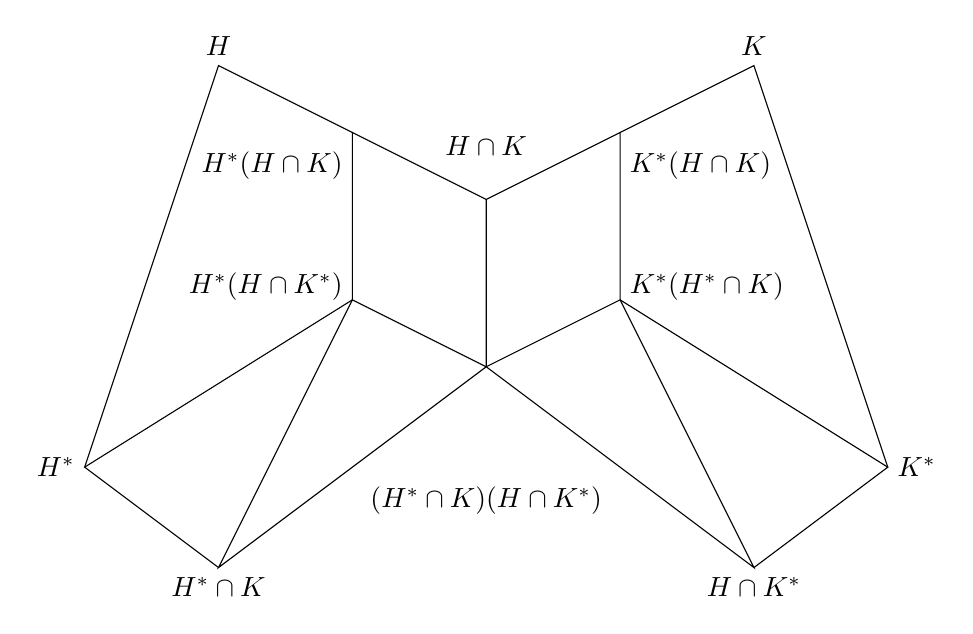
\begin{tikzpicture}[scale=1.7]

\draw  (0,0) -- (1,0.5) -- (2,-1.5) -- cycle;
\draw  (0,0) -- (0,1.25) -- (1,1.75) -- (1,0.5);
\draw (1,0.5) -- (3,-0.75) -- (2,-1.5) node [below] {$H \cap K^*$};
\draw (1,1.75) -- (2,2.25) node [above] {$K$} -- (3,-0.75) node [right] {$K^*$};
\node at (1, 0.6) [right] {$K^*(H^* \cap K)$};
\node at (1, 1.5) [right] {$K^*(H \cap K)$};


\draw  (0,0) -- (-1,0.5) -- (-2,-1.5) -- cycle;
\draw  (0,1.25) -- (-1,1.75) -- (-1,0.5);
\draw (-1,0.5) -- (-3,-0.75) -- (-2,-1.5) node [below] {$H^* \cap K$};
\draw (-1,1.75) -- (-2,2.25) node [above] {$H$} -- (-3,-0.75) node [left] {$H^*$};
\node at (-1, 0.6) [left] {$H^*(H \cap K^*)$};
\node at (-1, 1.5) [left] {$H^*(H \cap K)$};

\node at (0, -1) {$(H^* \cap K)(H \cap K^*)$};
\node at (0, 1.65) {$H \cap K$};

\end{tikzpicture}
\end{center}

\caption{The Zassenhaus Lemma}
\label{Butterfly}
\end{figure}
 
\item
\textbf{Schreier's Theorem.}\index{Schreier's Theorem}
Use the Zassenhaus Lemma to prove that two subnormal (normal) series 
of a group $G$ have isomorphic refinements.
 
 
\item
Use Schreier's Theorem to prove the  Jordan-H\"{o}lder Theorem.
 
\end{enumerate}
}
 
\subsection*{Programming Exercises}
 
{\small
Write a program that will compute all possible abelian
groups of order $n$.  What is the largest $n$ for which your
program will work?
}
 
 
 
\subsection*{References and Suggested Readings}  %%References checked and updated - TWJ 6/22/2010
 
{\small
Each of the following references contains a proof of the Fundamental
Theorem of Finitely Generated Abelian Groups.
\begin{itemize}
 
\item[\textbf{[1]}]   %%Reference updated 6/22/2010 - TWJ
Hungerford, T. W. 
\textit{Algebra}. Springer, New York, 1974. .
 
\item[\textbf{[2]}] %%Reference updated 6/22/2010 - TWJ
Lang, S. 
\textit{Algebra}. 3rd ed. Springer, New York, 2002.

 
\item[\textbf{[3]}] %%Reference updated 6/22/2010 - TWJ
Rotman, J. J. \textit{An Introduction to the Theory of
Groups}. 4th ed. Springer, New York, 1995.
 
 
\end{itemize}
}

\sagesection
 
 
 
 
